\section{导数控制}
\label{sec:sobolev-derivative-control}

$L^2$范数把函数在整个区间上的平方大小累加起来，它记录“有多大”，不记录“变化有多快”。本节在$(0,1)$上比较四类函数：频率不同的正弦、常数、带一个折点的函数和阶跃函数。正弦说明只看$L^2$会遗漏振荡，常数说明只看导数会遗漏高度，折点和跳跃则要求我们决定，哪些不能经典求导的函数仍应计入。

\subsection{振荡函数}
\label{sec:sobolev-oscillation}

对正整数$n$，取$f_n(x)=\sin(2\pi nx)$，$0<x<1$。先算它的$L^2$大小。由$\sin^2\theta=(1-\cos2\theta)/2$，而$\cos(4\pi nx)$在$(0,1)$上恰好走过$2n$个完整周期，积分为零，所以
\[
\lVert f_n\rVert_2^2=\int_0^1\sin^2(2\pi nx)\,\mathrm dx=\frac12.
\]
于是
\[
\lVert f_n\rVert_2=\frac1{\sqrt2},
\]
这个值与$n$无关。

导数的情形完全不同。经典导数是$f_n'(x)=2\pi n\cos(2\pi nx)$，同样的计算给出
\begin{equation}
\lVert f_n'\rVert_2=2\pi n\cdot\frac1{\sqrt2}=\sqrt2\,\pi n .
\label{eq:sobolev-oscillation-derivative}
\end{equation}
图~\ref{fig:sobolev-oscillation}把两件事放在一起：左边$f_1$与$f_4$的振幅相同、$L^2$长度相同，右边导数的$L^2$范数却随$n$线性增长。导数范数记录的是函数在单位长度内上下摆动的程度。

\begin{BookInlineFigure}
  \centering
  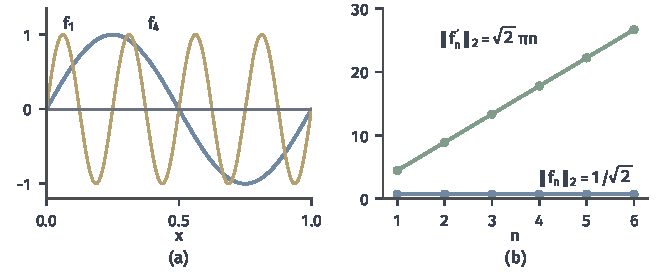
\includegraphics[width=112mm]{figures/04-spaces-measures-and-geometry/03-function-spaces/matplotlib/sobolev-oscillation/figure.pdf}
  \caption{振荡在$L^2$范数中不可见。(a)蓝色为$f_1$，黄色为$f_4$，其中$f_n(x)=\sin(2\pi nx)$，两者的$L^2$长度都是$1/\sqrt2$。(b)蓝点为$\lVert f_n\rVert_2$，保持不变；绿点为$\lVert f_n'\rVert_2$，按式~\eqref{eq:sobolev-oscillation-derivative}随$n$线性增长。}
  \label{fig:sobolev-oscillation}
\end{BookInlineFigure}

\paragraph{高频坐标上的权重}
用向量的语言重述这个现象。把$\sqrt2\sin(2\pi nx)$看成$L^2(0,1)$中的单位向量，它们两两正交，$f_n$就是沿第$n$条坐标轴、长度为$1/\sqrt2$的向量。求导把这条轴送到余弦轴上，同时把长度乘以$2\pi n$。所以频率越高的坐标，求导后放大得越多。

若把长度的平方改成“函数的平方加导数的平方”，第$n$条轴上的贡献就变成
\[
\lVert f_n\rVert_2^2+\lVert f_n'\rVert_2^2
=\frac12\bigl(1+(2\pi n)^2\bigr).
\]
这里的$1+(2\pi n)^2$就是一个权，高频坐标的权大，低频坐标的权小。把导数放进范数，相当于把各向同性的球压扁成沿高频方向很短的椭球。

有限维里可以把这件事完整算出来。取三个等距点上的取值$u=(u_1,u_2,u_3)$，用相邻差分$Du=(u_2-u_1,\ u_3-u_2)$代替导数。差分的平方和是一个二次型：
\[
\lVert Du\rVert^2=u^\top D^\top Du,\qquad
D^\top D=\begin{bmatrix}1&-1&0\\-1&2&-1\\0&-1&1\end{bmatrix}.
\]

这个矩阵的三个特征向量正好是三种“形状”，下面逐个验证。常向量$c=(1,1,1)$的相邻差为零，$D^\top Dc=0$，特征值是$0$。斜坡$t=(1,0,-1)$满足$D^\top Dt=t$，特征值是$1$。锯齿$z=(1,-2,1)$满足
\[
D^\top Dz=(3,-6,3)=3z,
\]
特征值是$3$。形状越“抖”，特征值越大。

于是在这组正交方向上，$\lVert u\rVert^2+\lVert Du\rVert^2$就是把三个坐标分别乘以权$1,2,4$再求和。以$z$为例：
\[
\lVert z\rVert^2=6,\qquad Dz=(-3,3),\qquad \lVert Dz\rVert^2=18=3\lVert z\rVert^2.
\]
函数空间的情形是同一幅图，只是坐标有无穷多个，权也趋于无穷。有限维时权总是有界的；无限维时权无界，这就是求导在$L^2$上不是有界算子的原因。

\paragraph{常数方向}
上面的权里常向量对应的导数项是零，这一点在函数上同样成立。常数函数$c$的导数为零，$\lVert c'\rVert_2=0$对每个$c$成立，只看导数无法区分$c=0$和$c=100$。导数度量变化，函数处在什么高度要由函数本身的大小记录。

所以完整的度量必须同时保留$\lVert f\rVert_2$和$\lVert f'\rVert_2$，也就是上面权里的“$1$”。只有附加零边界或零均值条件、排除了常数方向以后，导数才可能单独控制函数，这是第~\ref{sec:sobolev-derivative-norms}小节的问题。

\subsection{折点与跳跃}
\label{sec:sobolev-kinks-jumps}

若坚持经典导数，$f(x)=|x-1/2|$就会被排除：它只在$x=1/2$处没有导数，其余各点都光滑，变化速度恒为$1$。可是从“累积变化量”的角度看，这个函数没有任何异常。我们用第~\ref{chap:smoothing-weak-derivatives}章的弱导数来检查它。

令$g(x)=\operatorname{sgn}(x-1/2)$，即$x<1/2$时取$-1$，$x>1/2$时取$1$。任取测试函数$\varphi\in C_c^\infty(0,1)$，在折点两侧分别分部积分：
\[
\begin{aligned}
\int_0^1 f\varphi'\,\mathrm dx
&=\int_0^{1/2}\Bigl(\frac12-x\Bigr)\varphi'\,\mathrm dx
+\int_{1/2}^1\Bigl(x-\frac12\Bigr)\varphi'\,\mathrm dx\\
&=\int_0^{1/2}\varphi\,\mathrm dx-\int_{1/2}^1\varphi\,\mathrm dx
=-\int_0^1 g\varphi\,\mathrm dx .
\end{aligned}
\]
边界项在$x=1/2$处都含因子$f(1/2)=0$，在端点处$\varphi$为零，所以全部消失。按弱导数的定义，$f'=g$。

折点函数和它的弱导数都平方可积，大小可以直接算出：
\[
\lVert f\rVert_2^2=2\int_0^{1/2}t^2\,\mathrm dt=\frac1{12},\qquad
\lVert f'\rVert_2^2=1 .
\]
单点不能经典求导并不妨碍用$\lVert f\rVert_2$和$\lVert f'\rVert_2$同时控制它。把这类函数放在一起，就得到第~\ref{sec:sobolev-norms-completeness}节将记为$H^1(0,1)$的空间。

阶跃函数的情形不同。令$H=\mathbf 1_{[1/2,1)}$，对测试函数$\varphi$计算
\begin{equation}
-\int_0^1 H\varphi'\,\mathrm dx=-\int_{1/2}^1\varphi'\,\mathrm dx=\varphi(1/2).
\label{eq:sobolev-step-action}
\end{equation}
跳跃把测试函数送到它在跳跃点的取值，图~\ref{fig:sobolev-kink-step}的(d)画的就是这一作用。

\begin{BookInlineFigure}
  \centering
  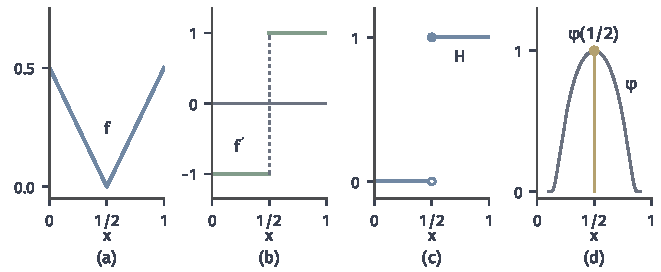
\includegraphics[width=112mm]{figures/04-spaces-measures-and-geometry/03-function-spaces/matplotlib/sobolev-kink-step/figure.pdf}
  \caption{折点与跳跃。(a)折点函数$f(x)=|x-1/2|$，连续。(b)它的弱导数$f'$，在$x=1/2$处跳跃，但仍是平方可积的函数。(c)阶跃函数$H$，在$x=1/2$处跳跃。(d)$H$对测试函数$\varphi$的作用只读取$\varphi(1/2)$，黄色竖线所示；这一作用集中在一点，不是任何函数的积分。}
  \label{fig:sobolev-kink-step}
\end{BookInlineFigure}

这个作用不能写成函数的积分。假设有局部可积函数$h$使$\int_0^1h\varphi\,\mathrm dx=\varphi(1/2)$对所有测试函数成立。对支撑不含$1/2$的$\varphi$，右端是零，由测试函数判别，$h$在$(0,1/2)$和$(1/2,1)$上都几乎处处为零。于是$h=0$几乎处处，而这与取$\varphi(1/2)\neq0$的测试函数矛盾。所以$H$没有弱导数，不属于上述空间。

阶跃函数在$x\neq1/2$处的经典导数是零，所以几乎处处导数是$0$。但$0$并不是它的弱导数，否则$H$几乎处处为常数。这个例子提醒我们，Sobolev空间中的“导数”始终指弱导数，几乎处处存在的经典导数不能自动代替它。

\paragraph{用余弦坐标比较}
现在把这些例子放到同一组坐标里。在$L^2(0,1)$上取正交归一基
\begin{equation}
e_0(x)=1,\qquad e_n(x)=\sqrt2\cos(\pi nx)\quad(n\geq1).
\label{eq:sobolev-cosine-basis}
\end{equation}
它是把函数偶延拓到$(-1,1)$后的Fourier基，完备性来自第~\ref{chap:fourier-transform}章。函数$f$的坐标是$a_n=\int_0^1fe_n\,\mathrm dx$，Parseval等式给出$\lVert f\rVert_2^2=\sum_na_n^2$。选用余弦基的原因在第~\ref{sec:sobolev-hk}小节说明。

先算折点函数的坐标。$f$关于$x=1/2$对称，而$n$为奇数时$\cos(\pi nx)$关于$x=1/2$反对称，所以奇数项为零。取$n=2m$，分部积分得
\[
\int_0^{1/2}\Bigl(\frac12-x\Bigr)\cos(2\pi mx)\,\mathrm dx
=\frac{1-\cos(\pi m)}{(2\pi m)^2}.
\]
因此$a_0=1/4$，而$n=2m$时
\[
a_{2m}=\frac{\sqrt2}{\pi^2m^2}\quad(m\text{为奇数}),\qquad
a_{2m}=0\quad(m\text{为偶数}).
\]

再算阶跃函数的坐标。$a_0=1/2$，$n\geq1$时直接积分得
\[
a_n=\sqrt2\int_{1/2}^1\cos(\pi nx)\,\mathrm dx
=-\frac{\sqrt2\,\sin(\pi n/2)}{\pi n}.
\]
所以偶数项为零，奇数项的绝对值是$\sqrt2/(\pi n)$。折点的坐标按$1/n^2$衰减，阶跃的坐标只按$1/n$衰减。

把坐标乘上权$\pi^2n^2$后求部分和，令$S_N=\sum_{n\leq N}\pi^2n^2a_n^2$。折点函数只有$n=2m$（$m$为奇数）的项，每项是
\[
\pi^2(2m)^2\cdot\frac{2}{\pi^4m^4}=\frac{8}{\pi^2m^2},
\]
再用$\sum_{m\text{奇}}m^{-2}=\pi^2/8$，得到$S_N\to1$，恰好等于$\lVert f'\rVert_2^2$。

阶跃函数的每个奇数项都是
\[
\pi^2n^2\cdot\frac{2}{\pi^2n^2}=2,
\]
所以$S_N$随$N$线性增长，趋于无穷。图~\ref{fig:sobolev-cosine-coordinates}对比了这两条路径：折点函数的加权和收敛到$1$，阶跃函数的加权和发散。

\begin{BookInlineFigure}
  \centering
  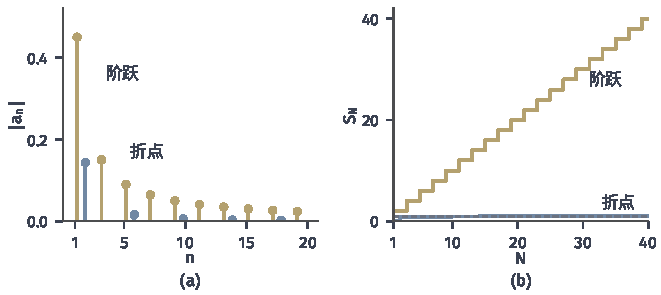
\includegraphics[width=112mm]{figures/04-spaces-measures-and-geometry/03-function-spaces/matplotlib/sobolev-cosine-coordinates/figure.pdf}
  \caption{折点与阶跃的余弦坐标。蓝色为折点函数$|x-1/2|$，黄色为阶跃函数$\mathbf 1_{[1/2,1)}$。(a)坐标的绝对值$|a_n|$，$n\geq1$。(b)加权部分和$S_N=\sum_{n\leq N}\pi^2n^2a_n^2$，虚线高度为$1$，折点的部分和收敛到这一高度，阶跃的部分和线性增长。}
  \label{fig:sobolev-cosine-coordinates}
\end{BookInlineFigure}

这就是用坐标看到的结论：Sobolev范数有限，等于坐标在加权后仍然平方可和。至于阶跃这样的跳跃应当怎样按尺度度量，第~\ref{chap:besov-spaces}章会用平移差回答。
